\section{Correlation Analysis}
A correlation analysis between the spectrogram and the cepstrogram coefficients has been performed by the following code
\begin{lstlisting}
frame = 100;

[c_spectra,rho1] = corr(log10(spectgram_f(:,1:frame)).');
[c_cepstra,rho2] = corr(mfccs_f(:,1:frame).');
figure(11)
subplot(1,2,1); imagesc(abs(c_spectra)); title('Correlation - Female voice');...
    xlabel('Frequency bins'); ylabel('Frequency bins');
subplot(1,2,2); imagesc(abs(c_cepstra)); title('Correlation - Female voice');...
    xlabel('Cepstral Coefficient'); ylabel('Cepstral Coefficient');
\end{lstlisting}

Figure \ref{fig:11} shows the absolute values and it is visible, that the MFCC coefficients are less correlated since the matrix is more diagonal (the area outside the diagonal is much darker in the cepstogram, which means weaker intensity).\\While elements adjacent to the diagonal elements have a correlation value between approximately $0$ and $0.4$, the spectral correlation have mostly a much higher correlation, especially for the frequency bins 150 to 400. Figure \ref{fig:11_gray} shows the same picture with the \textit{gray colormap}, which supports the previous statement.

\begin{figure}[h]
		\centering
	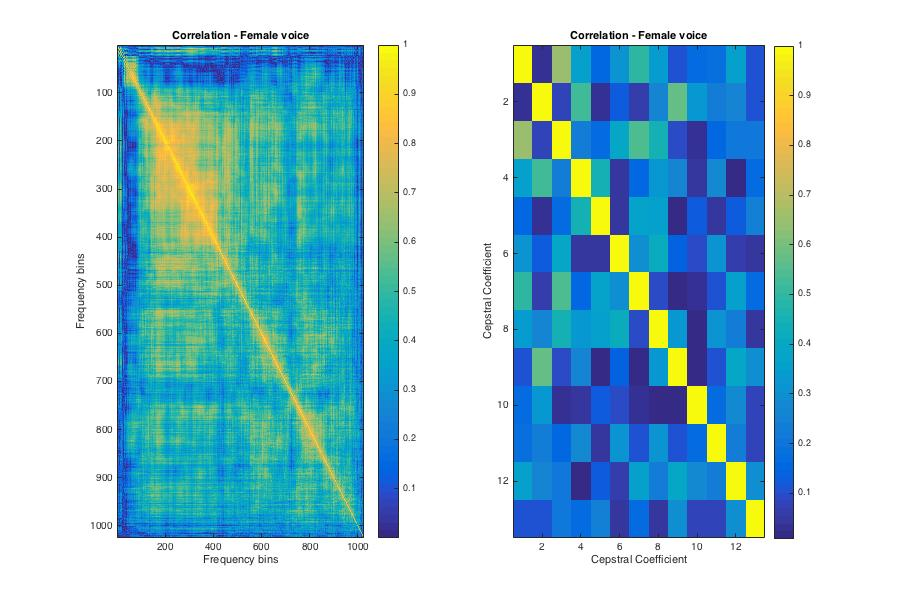
\includegraphics[width=0.75\linewidth]{./images/11.jpg}
		\caption{Coefficient correlation analysis}
		\label{fig:11}	
\end{figure}

\begin{figure}[h]
		\centering
		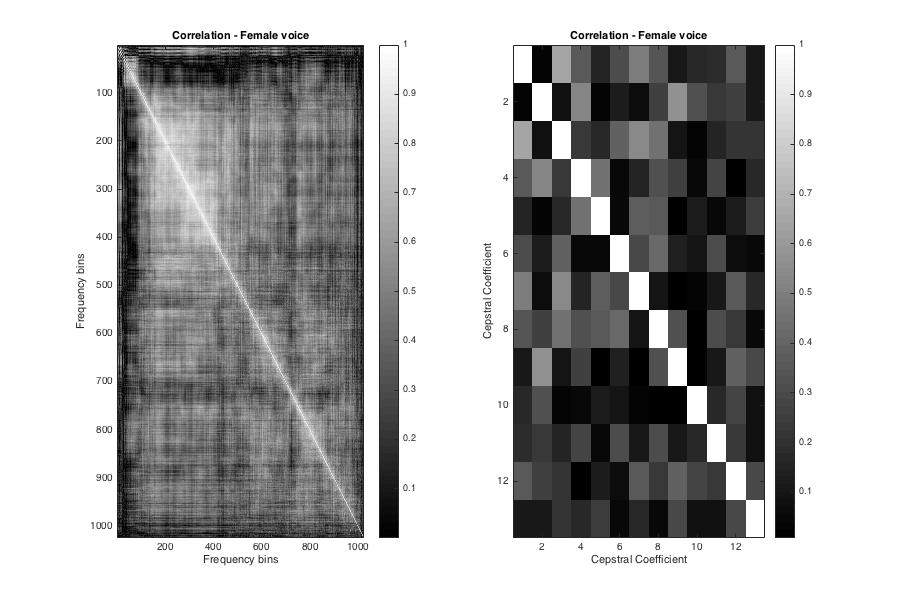
\includegraphics[width=0.75\linewidth]{./images/11_gray.jpg}
		\caption{Coefficient correlation analysis (gray colormap)}
		\label{fig:11_gray}	
\end{figure}
